\documentclass[a4paper,12pt]{article}
\usepackage{graphicx}
\usepackage{geometry}
\geometry{margin=1in}

\begin{document}

% ─────────────────────────────────────────────
% Title Page
% ─────────────────────────────────────────────
\begin{titlepage}
    \centering
    \vspace*{3cm}
    {\Huge \bfseries Reinforcement Learning: \\ Setting Up Gymnasium Environments \par}
    \vspace{2cm}
    {\Large \textit{Lab 1 Task Report} \par}
    \vspace{3cm}
    {\large \textbf{Submitted by:} \\ Junaid Asif \par}
    \vspace{0.5cm}
    {\large \textbf{Roll No:} BSAI-144 \par}
    \vspace{0.5cm}
    {\large \textbf{Instructor:} \par}
    \vfill
    {\large February 20, 2026 \par}
\end{titlepage}

% ─────────────────────────────────────────────
% Step 1: requirements.txt
% ─────────────────────────────────────────────
\begin{figure}[h!]
    \centering
    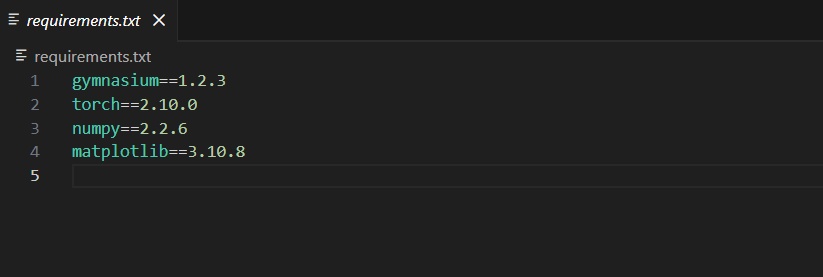
\includegraphics[width=\textwidth]{requirements.png}
    \caption{requirements.txt with pinned library versions}
\end{figure}

% ─────────────────────────────────────────────
% Step 2: Installed Packages
% ─────────────────────────────────────────────
\begin{figure}[h!]
    \centering
    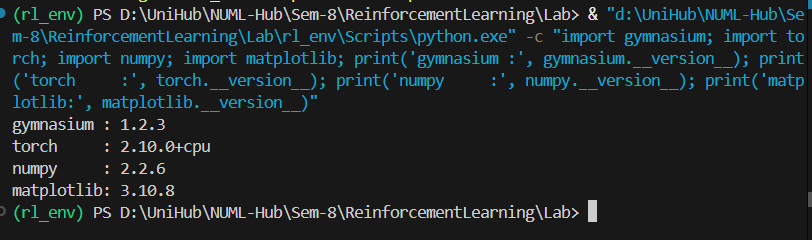
\includegraphics[width=\textwidth]{InstalledPackages.png}
    \caption{Installed packages verification (pip list)}
\end{figure}

\newpage

% ─────────────────────────────────────────────
% Environment 1: CartPole-v1
% ─────────────────────────────────────────────
\begin{figure}[h!]
    \centering
    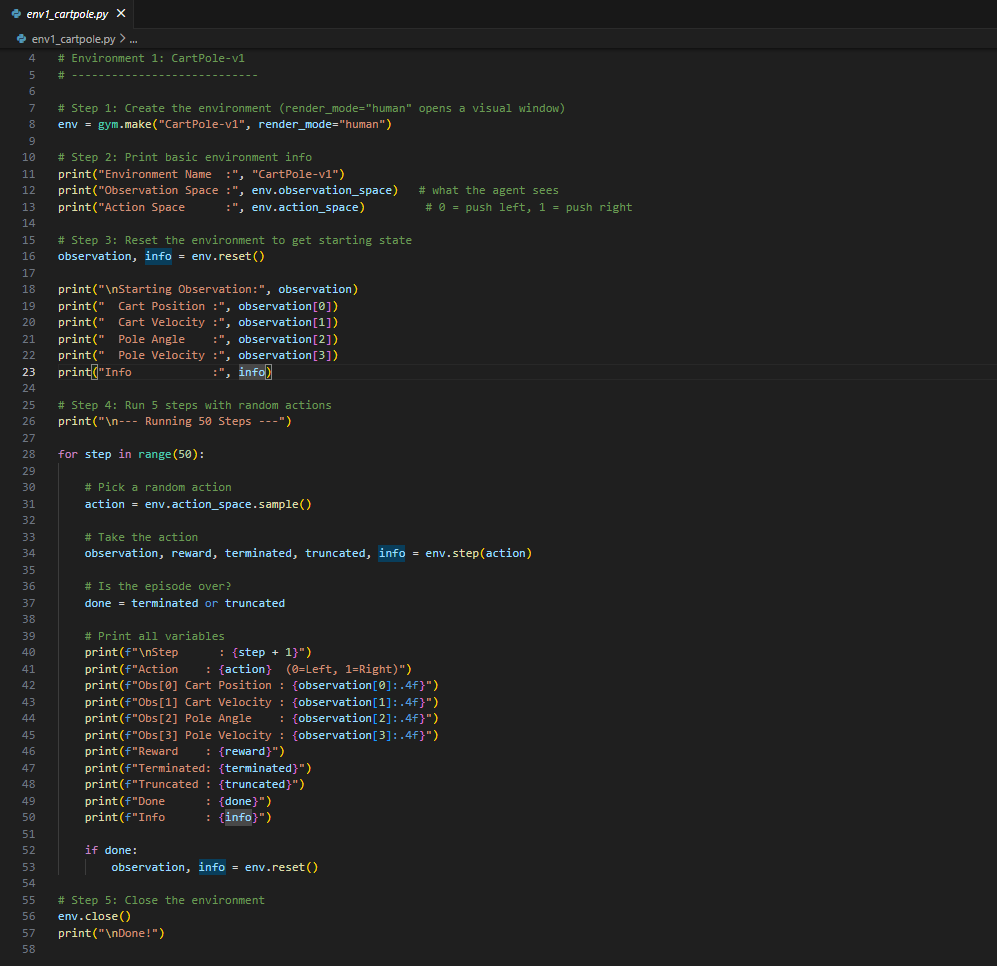
\includegraphics[width=\textwidth]{CartpoleCode.png}
    \caption{CartPole-v1 -- Python code}
\end{figure}

\begin{figure}[h!]
    \centering
    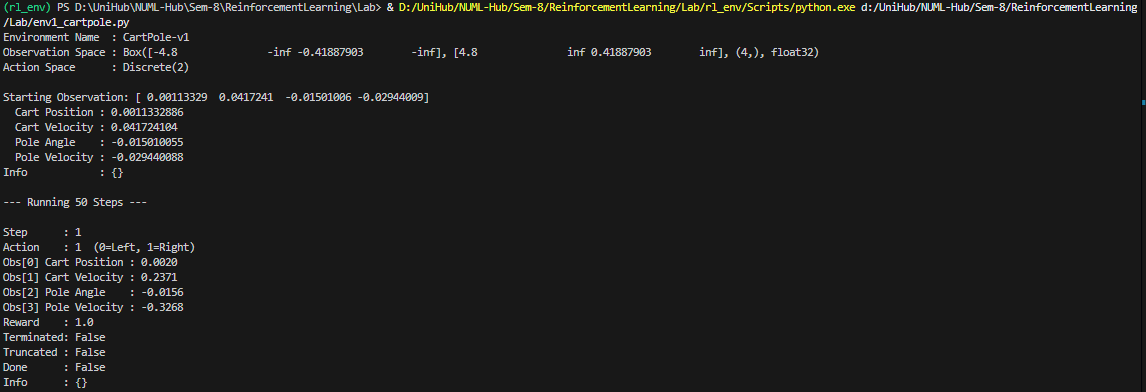
\includegraphics[width=\textwidth]{CartpoleOutput.png}
    \caption{CartPole-v1 -- Terminal output showing all variable values}
\end{figure}

\begin{figure}[h!]
    \centering
    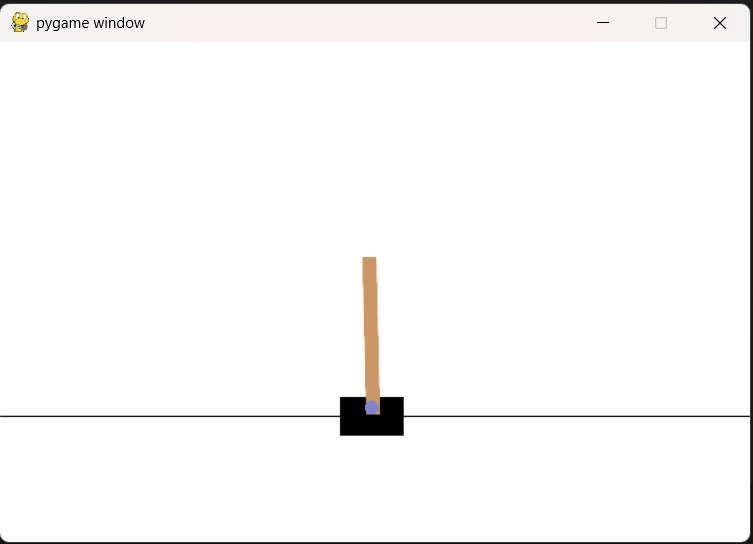
\includegraphics[width=0.75\textwidth]{CartpoleFig.png}
    \caption{CartPole-v1 -- Visual render window}
\end{figure}

\newpage

% ─────────────────────────────────────────────
% Environment 2: FrozenLake-v1
% ─────────────────────────────────────────────
\begin{figure}[h!]
    \centering
    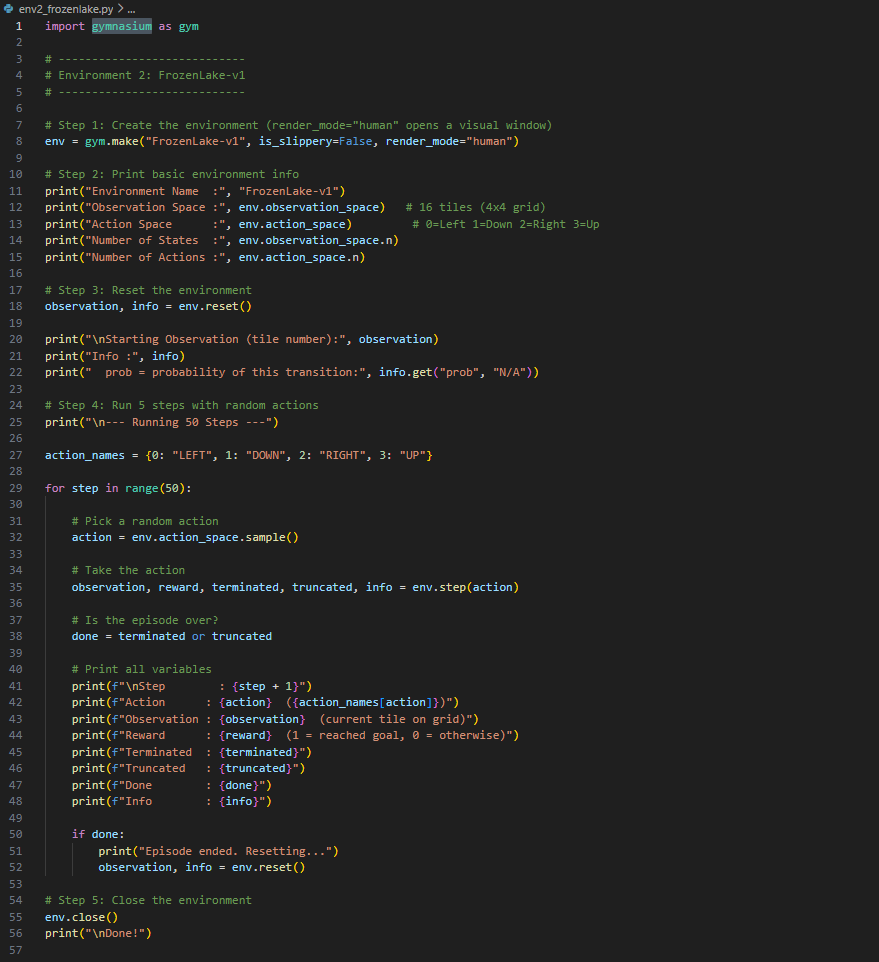
\includegraphics[width=\textwidth]{FrozenlakeCode.png}
    \caption{FrozenLake-v1 -- Python code}
\end{figure}

\begin{figure}[h!]
    \centering
    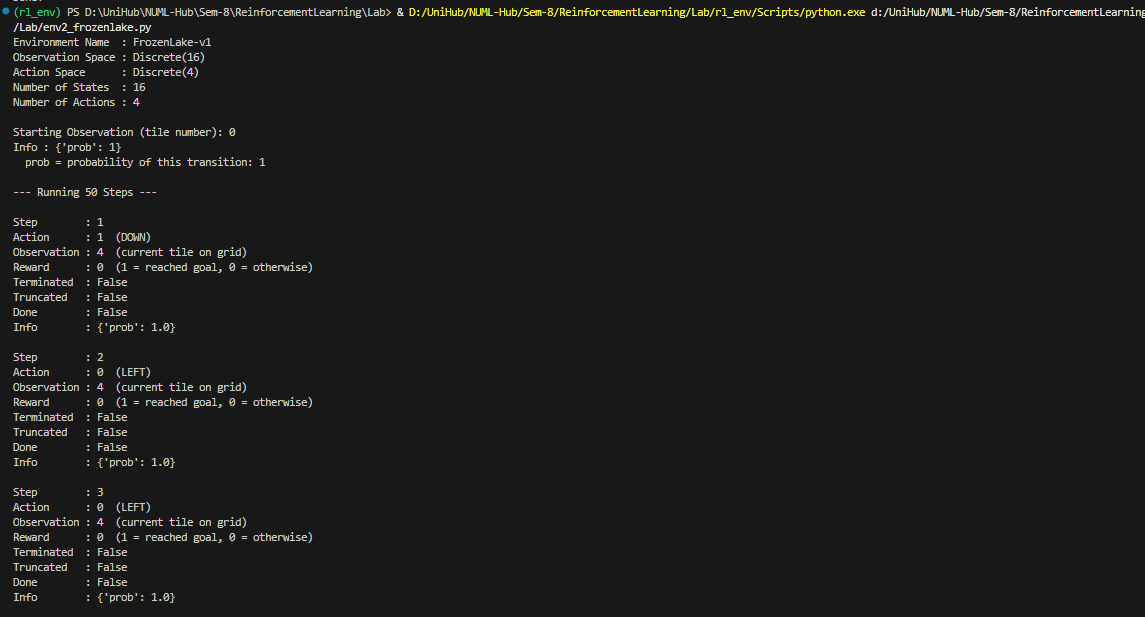
\includegraphics[width=\textwidth]{FrozenlakeOutput.png}
    \caption{FrozenLake-v1 -- Terminal output showing all variable values}
\end{figure}

\begin{figure}[h!]
    \centering
    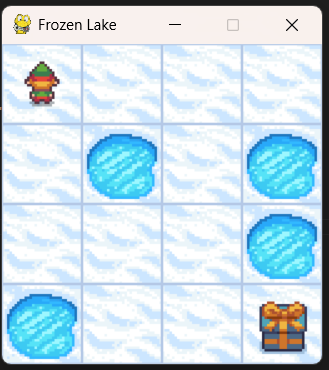
\includegraphics[width=0.75\textwidth]{FrozenlakeFig.png}
    \caption{FrozenLake-v1 -- Visual render showing the 4x4 grid}
\end{figure}

\newpage

% ─────────────────────────────────────────────
% Environment 3: MountainCar-v0
% ─────────────────────────────────────────────
\begin{figure}[h!]
    \centering
    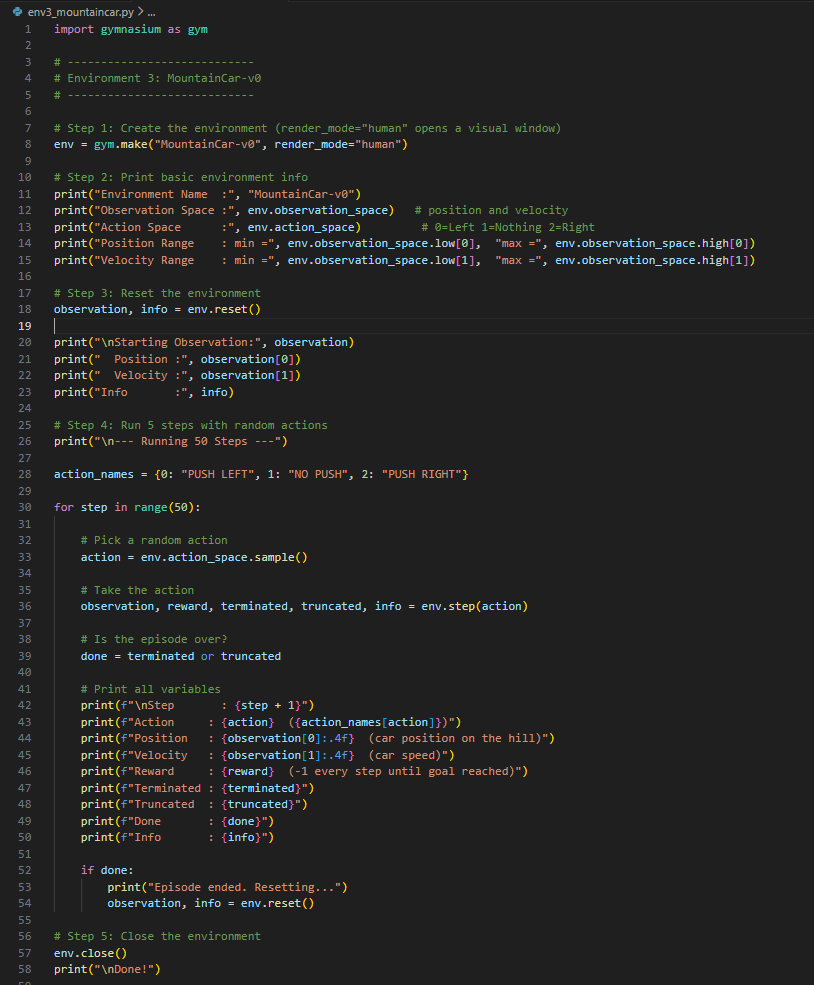
\includegraphics[width=\textwidth]{MountaincarCode.png}
    \caption{MountainCar-v0 -- Python code}
\end{figure}

\begin{figure}[h!]
    \centering
    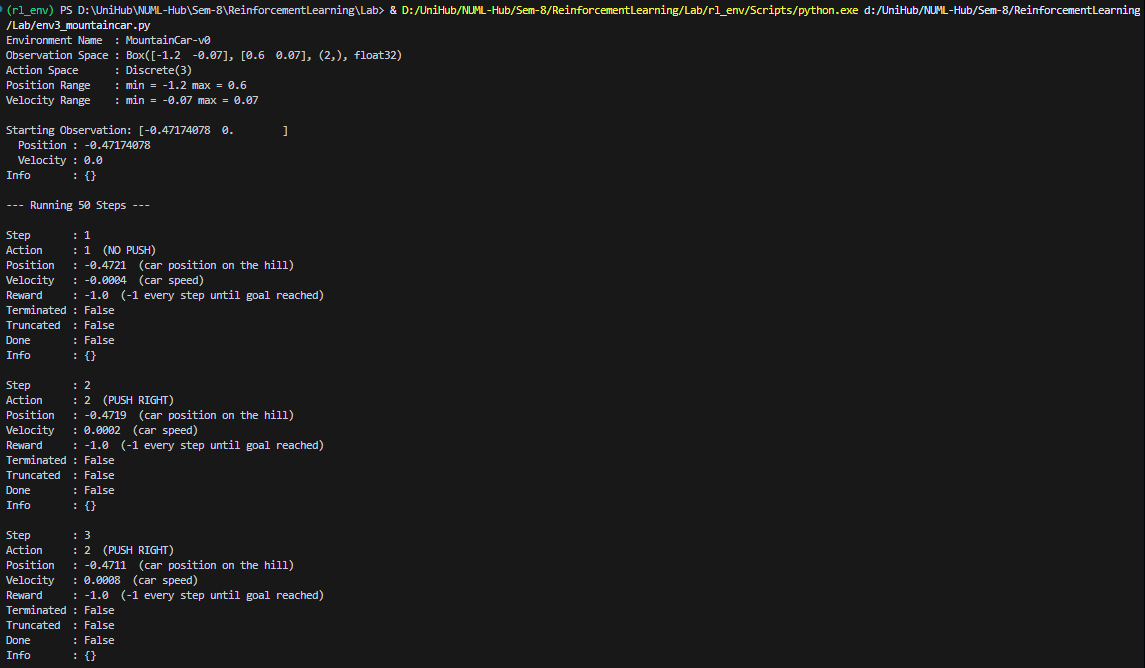
\includegraphics[width=\textwidth]{MountaincarOutput.png}
    \caption{MountainCar-v0 -- Terminal output showing all variable values}
\end{figure}

\begin{figure}[h!]
    \centering
    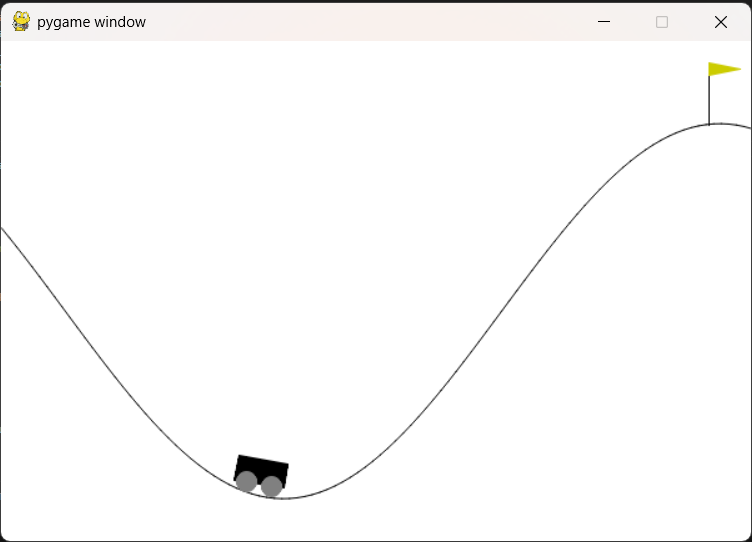
\includegraphics[width=0.75\textwidth]{MountaincarFig.png}
    \caption{MountainCar-v0 -- Visual render showing the car on the hill}
\end{figure}

\end{document}
